\section*{Question 5:}
Exercise 7.2: 

Can you think of another measure of similarity that could be used in the vector space model? Compare your measure with the cosine correlation using some example documents and queries with made-up weights. Browse the IR literature on the Web and see whether your measure has been studied (start with van Rijsbergen’s book).

\subsection*{Answer:}

In order for the similarity measure to be correct and accurate when used in the vector space model, it must be based on the angle between the two vectors. Any measure that is based on the Euclidean distance will give wrong results unless both vectors, query \& document vectors, are reduced to the unit vectors, which is what cosine similarity does.

\textbf{Example:}

We have a query q = ``Do jealous people gossip?''. Let's assume that the two terms ``do'' and ``people'' are stop words. The two terms that affect the results are ``jealous'' and ``gossip''.

We also have three documents to examine, $d_1$, $d_2$, and $d_3$.

$d_1$: A document that is mostly about gossip, but has a little about jealousy.

$d_2$: A document about both gossip and jealousy. It has a little more about jealousy than it does about gossip. It the most relevant document out of all three documents.

$d_3$: A document that is mostly about jealousy, but has a little about gossip.

Euclidean distance similarity will cause $d_1$ and $d_3$ to be ranked higher than $d_2$ with respect to the query q because the distance between q and $d_2$ is larger than the distance between q and $d_1$ as well as the distance between q and $d_3$. The result is clear in Figure 1

\begin{figure}[h]
\caption{Euclidean Distance Similarity}
\centering
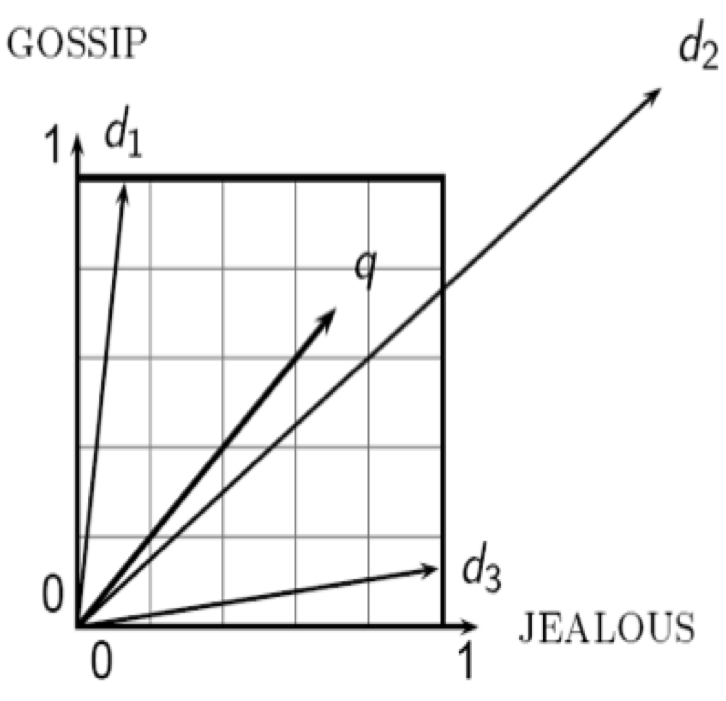
\includegraphics[scale=0.4]{Q5/cosine.png}
\end{figure}


The only case where Euclidean distance can be used as a similarity measure is when all vectors are reduced to the unit vector. This reduction can be performed by dividing each component in the vector by the vector's magnitude. The result is clear in Figure 2

\begin{figure}[h]
\caption{Euclidean Distance Similarity Between Unit Vectors}
\centering
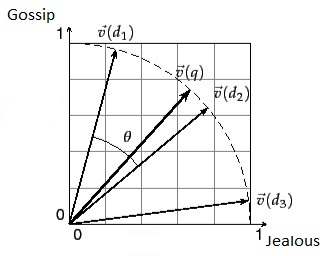
\includegraphics[scale=0.7]{Q5/cosinesimilarity.jpg}
\end{figure}

Cotangent of the angle between vectors could be used as a measure of similarity in the vector space model. Cotangent $\theta$ is the reciprocal of tangent $\theta$. The graph of the function $y = cot(x)$ is shown in Figure 3.

\begin{figure}[h]
\caption{Euclidean Distance Similarity Between Unit Vectors}
\centering
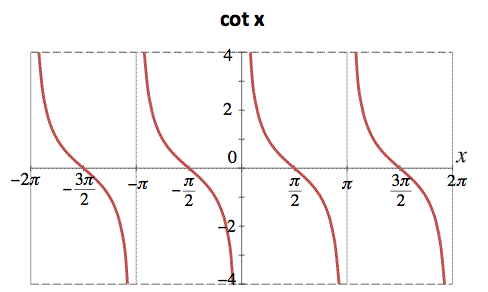
\includegraphics[scale=1.1]{Q5/graph_cot_pi.png}
\end{figure}

The period of the function cotangent that should be used lies in the interval $\theta = [0,\pi]$

From the graph, three statements can be made:

1. If the angle between the vectors is zero, the value of the cotangent is $\infty$.

2. If the angle between the vectors is $\frac{\pi}{2}$, the value of the cotangent is zero.

3. If the angle between the vectors is $\pi$, the value of the cotangent is $-\infty$.

This similarity measure agrees with the cosine similarity measure, but it is very steep since its value spans the interval $(-\infty,+\infty)$.

The log function can be wrapped around the cotangent function to reduce its aggression. 

$ similarity = \log_{10} (\cot(\theta))$

The base of the log is not important. Base 10 is not empirically determined. The base is there for completeness.



 
